%%%%%%%%%%%%%%%%%%%%%%%%%%%%%%%%%%%%%%%%%
% University Assignment Title Page 
% LaTeX Template
% Version 1.0 (27/12/12)
%
% This template has been downloaded from:
% http://www.LaTeXTemplates.com
%
% Original author:
% WikiBooks (http://en.wikibooks.org/wiki/LaTeX/Title_Creation)
%
% License:
% CC BY-NC-SA 3.0 (http://creativecommons.org/licenses/by-nc-sa/3.0/)
% 
% Instructions for using this template:
% This title page is capable of being compiled as is. This is not useful for 
% including it in another document. To do this, you have two options: 
%
% 1) Copy/paste everything between \begin{document} and \end{document} 
% starting at \begin{titlepage} and paste this into another LaTeX file where you 
% want your title page.
% OR
% 2) Remove everything outside the \begin{titlepage} and \end{titlepage} and 
% move this file to the same directory as the LaTeX file you wish to add it to. 
% Then add \input{./title_page_1.tex} to your LaTeX file where you want your
% title page.
%
%%%%%%%%%%%%%%%%%%%%%%%%%%%%%%%%%%%%%%%%%
%\title{Title page with logo}
%----------------------------------------------------------------------------------------
%	PACKAGES AND OTHER DOCUMENT CONFIGURATIONS
%----------------------------------------------------------------------------------------

\documentclass[12pt]{article}
\usepackage[english]{babel}
\usepackage[utf8x]{inputenc}
\usepackage{amsmath}
\usepackage{graphicx}
\usepackage[colorinlistoftodos]{todonotes}
\usepackage{hyperref}
\usepackage{float}
\usepackage{caption}
\usepackage{subcaption}


\begin{document}

\begin{titlepage}

\newcommand{\HRule}{\rule{\linewidth}{0.5mm}} % Defines a new command for the horizontal lines, change thickness here

\center % Center everything on the page
 
%----------------------------------------------------------------------------------------
%	HEADING SECTIONS
%----------------------------------------------------------------------------------------

\textsc{\LARGE Università degli studi di Milano-Bicocca}\\[1cm] % Name of your university/college
\textsc{\Large Advanced Machine Learning }\\[0.3cm] % Major heading such as course name
\textsc{\large Progetto finale}\\[0.1cm] % Minor heading such as course title

%----------------------------------------------------------------------------------------
%	TITLE SECTION
%----------------------------------------------------------------------------------------

\HRule \\[0.4cm]
{ \huge \bfseries Fruit Recognition Project}\\[0.4cm] % Title of your document
\HRule \\[1.5cm]
 
%----------------------------------------------------------------------------------------
%	AUTHOR SECTION
%----------------------------------------------------------------------------------------

\large
\emph{Autore:}\\
Andrea Guzzo - 761818 - a.guzzo1@campus.unimib.it    % Your name
 \\[1cm] 

% If you don't want a supervisor, uncomment the two lines below and remove the section above
%\Large \emph{Author:}\\
%John \textsc{Smith}\\[3cm] % Your name

%----------------------------------------------------------------------------------------
%	DATE SECTION
%----------------------------------------------------------------------------------------

Luglio 2019\\[2cm] % Date, change the \today to a set date if you want to be precise

%----------------------------------------------------------------------------------------
%	LOGO SECTION
%----------------------------------------------------------------------------------------


\includegraphics{logo.png}\\[1cm] % Include a department/university logo - this will require the graphicx package
 
%----------------------------------------------------------------------------------------

\vfill % Fill the rest of the page with whitespace

\end{titlepage}


\begin{abstract}
Nel mondo del Deep Learning esistono molte tecniche per la creazione di reti neurali in grado di riconoscere oggetti a partire da immagini.  
La soluzione proposta vuole quindi fare una panoramica di possibili tecniche e differenti soluzioni volte alla realizzazione di una rete neurale in grado di riconoscere differenti tipi di frutta all'interno di immagini.
L'utilizzo di diversi approcci ha permesso il confronto, l'identificazione e la sperimentazione di alcune pratiche illustrate all'interno del documento per fornire in ultima istanza alcuni suggerimenti e consigli sull'utilizzo delle tecniche e metodologie trattate.
\end{abstract}

\section{Introduzione}
Nel corso degli ultimi anni, il riconoscimento di oggetti all'interno di immagini è diventato un task comune e di più semplice risoluzione rispetto al passato.
Grazie all'aumentare della potenza di calcolo disponibile, a nuovi tipi di architetture di reti neurali Deep, ad algoritmi sempre più efficienti implementati da framework di facile utilizzo e comprensione,è possibile ottenere delle ottime performance a partire da datasets disponibili gratuitamente online, adattando le soluzioni realizzate in modo sempre meno complesso ai differenti casi d'uso.  
A tal proposito per comprendere l'uso delle differenti tecniche e per sperimentare alcuni dei diversi approcci che è possibile adottare, per addestrare delle reti neurali in grado di riconoscere oggetti all'interno di immagini più o meno complesse, è stato realizzato uno studio contenente tre metodologie di lavoro differenti:
\begin{enumerate}
\item addestramento di reti neurali utilizzando tecniche di Transfer Learning \cite{transferlearning}
\item utilizzo di tecniche di Layer Freezing per creare strutture personalizzate a partire da reti neurali esistenti
\item implementazione di un algoritmo convoluzionale progettato da zero.
\end{enumerate}

Il confronto tra questi tre differenti approcci, sia in termini di performance, che in termini di velocità di realizzazione e di training ha permesso di delineare alcune pratiche di uso comune, alcune strategie che possono essere facilmente adattate in progetti di più larga complessità su tasks simili.  
Come ultimo risultato del lavoro svolto, sono stati analizzati e discussi differenti approcci di rilascio e organizzazione delle architetture per consentire la messa in produzione di algoritmi previsionali in ambito Deep Learning.


\section{Dataset}
Per il progetto è stato utilizzato un dataset disponibile gratuitamente all'interno della piattaforma: Kaggle chiamato: moltean fruits 360 dataset \cite{dataset}
Questa collezione di dati viene spesso utilizzata per confrontare tecniche di Deep Learning, per studiare e confrontare approcci e metodi differenti.
È composto da un numero di immagini totale pari a: 71125, con un traininset diviso in 53177 immagini contenti un frutto per ogni immagine con dimensione per ogni immagine di 100x100 pixels.  
Il validation set contiene al suo interno 17845 immagini sempre rappresentati un frutto per ogni immagine, mentre è presente all'interno dei dati disponibile anche un set di immagini contenente 103 immagini dove è possibile trovare più di un frutto all'interno di ogni singola immagine.  
Il numero di classi all'interno dei dati al momento dell'utilizzo e del progetto è di 103 classi differenti, ognuna appartenente ad un frutto differente.  
Il dataset non è comprensivo di tutti i tipi di frutta esistenti e viene costantemente aggiornato e arricchito. \\
Il progetto dunque assume che la numerosità delle classi all'interno del dataset sia sufficiente a coprire la maggior parte delle casistiche di frutti comunemente venduti in commercio e disponibili.  \\
La particolarità di questo dataset è che sono disponibili una sequenza di immagini per ogni frutto ottenute con una serie di fotografie scattate in sequenza che consentono la visione del frutto da diversi tipi di angolazione.  
  
 Per favorire l'apprendimento delle reti neurali utilizzate, sono state applicate anche differenti trasformazioni al dataset:
 
\begin{itemize}
\item operazioni di ridimensionamento 
\item operazioni di data augmentation
\end{itemize}

Le operazioni di ridimensionamento implementate all'interno di funzioni generiche hanno consentito il facile ridimensionamento delle immagini in modo da adattare l'input necessario alle differenti architetture di reti neurali utilizzate.  
Per la data augmentation è stato implementato un metodo che consente la generazione e la manipolazione a partire da immagini esistente, generando una sequenza di immagini con differenti attributi a partire da quelle di partenza: con differente orientamento, applicando zoom, rotazioni e spostamenti.  
La generazione di immagini a partire da quelle esistenti è una procedura comunemente nota che consente di manipolare il dataset di partenza per aggiungere nuovi record per il training degli algoritmi. \cite{dataaugmentation}  
Grazie alla buona qualità del dataset disponibile non è stato necessario eseguire alcun tipo di data cleaning e organizzazione delle informazioni.  
È stato comunque realizzato un connettore che consente il download e il setup automatico del dataset utilizzato a partire da Kaggle, sfruttando le kaggle API. \bigskip
Le reti neurali convoluzionali pre-trainate sono state selezionate in quanto utilizzano come dataset di riferimento ImageNet che contiene al suo interno immagini e classi simili a quelle presenti nel dataset considerato.  

\begin{figure}[H]
    \centering
    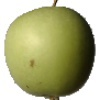
\includegraphics[width=0.2\textwidth]{./resources/mela.jpg}
    \caption{Immagine del dataset appartenente alla classe: apple golden 1} 
    \label{fig:mela}
\end{figure}

\begin{figure}[H]
    \centering
    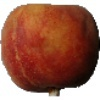
\includegraphics[width=0.2\textwidth]{./resources/pesca.jpg}
    \caption{Immagine del dataset appartenente alla classe: peach} 
    \label{fig:pesca}
\end{figure}

\begin{figure}[H]
    \centering
    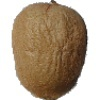
\includegraphics[width=0.2\textwidth]{./resources/kiwi.jpg}
    \caption{Immagine del dataset appartenente alla classe: kiwi} 
    \label{fig:kiwi}
\end{figure}

\section{Approccio metodologico}

Per raggiungere l'obiettivo del progetto, ovvero la sperimentazione e la validazione di differenti tecniche e approcci per la classificazione delle immagini sono stati effettuati tre tipi di esperimenti.  
Per effettuare tali sperimentazioni è stata impiegata una singola e determinata architettura hardware che ha permesso di effettuare il training e la validazione degli algoritmi impiegati.  
Tutti i benchmark, analisi, prototipazione e training sono stati effettuati utilizzando python, keras come framework di riferimento basato su tensorflow GPU versione 1, una scheda video Nvidia GTX1070 con 8 gb di vram, 16 gb di ram del sistema e un processore i5-8300.  
Il codice realizzato è disponibile su github al seguente indirizzo:  \url{https://github.com/JeyDi/FruitRecognition} \bigskip

Il Transfer Learning è una tecnica largamente utilizzata nel mondo del Deep learning, diventando uno strumento chiave nel mondo delle applicazioni di intelligenza artificiale, in particolare nelle aree di Computer Vision, Natural Language Processing, Speech Recognition, consentendo di produrre risultati determinanti sia in termini di performance, sia in termini di adattamento che di velocità di messa in produzione.  
La chiave di questo tipo di modelli è appunto la facilità di realizzazione di modelli accurati in un tempo significativo.  
Elemento fondamentale di questo approccio è il riutilizzo di modelli pre-trainati, ovvero modelli di Deep Learning che sono stati addestrati su dataset simili per compiere tasks che si avvicinano a quelli da implementare.  
Un algoritmo in grado di compiere il riconoscimento di oggetti all'interno di immagini sfrutta come tipologia di architettura delle reti neurali convoluzionali solitamente dotate di uno schema architetturale comune: un input definito, una base convoluzionale che consente di eseguire una fase di feature extraction a partire dalle immagini e successivamente un classificatore in grado di classificare correttamente le immagini in base alle classi considerate per arrivare ad una predizione quanto più veritiera possibile. 

\begin{figure}[H]
    \centering
    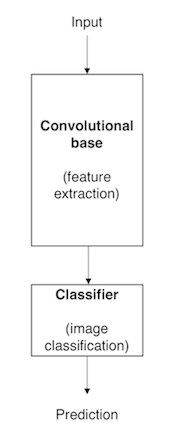
\includegraphics[width=0.2\textwidth]{./resources/CNNArchitecture.png}
    \caption{Architettura di una CNN} 
    \label{fig:cnn_architecture}
\end{figure}

\begin{figure}[H]
    \centering
    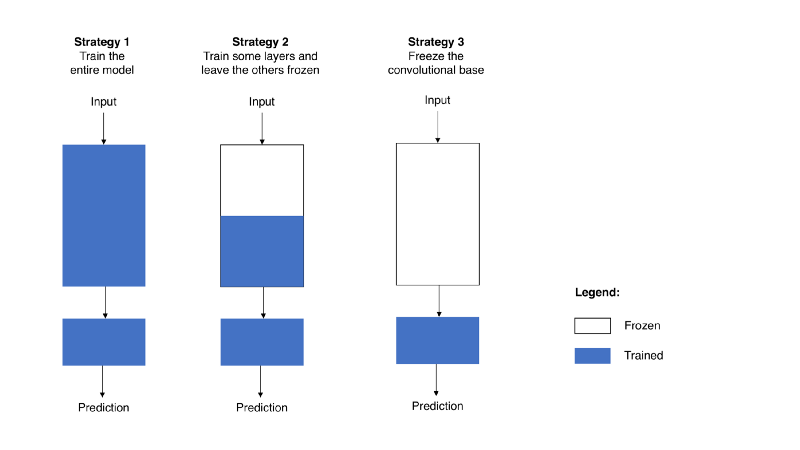
\includegraphics[width=1\textwidth]{./resources/transferLearningStrategies.png}
    \caption{Strategie di transfer learning} 
    \label{fig:transfer_learning_strategies}
\end{figure}

Il numero di layers e di nodi all'interno della base convoluzionale può variare a seconda del tipo di architettura e ovviamente questo esempio vuol solamente essere una semplificazione rispetto all'implementazione reale di una rete neurale convoluzionale.  
Una volta ottenuta una rete convoluzionale pre-trainata su un dataset e su un task simile si procede all'inserimento all'interno dell'architettura il proprio classificatore che consente di riconoscere le nuove immagini in input che verranno utilizzate rispetto alle nuove classi definite.  
Per fare questo si possono adottare tre tipi di approcci:
\begin{enumerate}
\item Fare il training dell'intero modello
\item Fare il training di alcuni layers, lasciando alcuni layer in stato frozen
\item Fare il freeze della base convoluzionale ritrainando solamente alcuni layer della parte convoluzionale
\end{enumerate}
  
Ognuno di questi approcci ha alcuni vantaggi e svantaggi, negli esperimenti trattati è stato compiuto un esperimento per l'approccio 1 e un esperimento per l'approccio 2. \bigskip

Per valutare l'efficacia di ogni esperimento realizzato e valutarne le performance al fine di selezionare l'approccio più conveniente in termini di sviluppo è stato adottato il seguente criterio di scelta:  
\begin{itemize}
\item analisi delle performance del modello
\item difficoltà di implementazione
\item tempo di training
\end{itemize}
Grazie all'analisi di questi parametri è stato possibile determinare quale approccio fosse più conveniente per compiere task simili.  
\bigskip

Successivamente all'implementazione e al training dei modelli si è anche scelto di salvare i modelli in formato ONNX in modo da esportare le reti addestrate anche su altri framework e per predisporre il rilascio della soluzione attraverso esperimenti dedicati di predizioni all'arrivo di nuove immagini. 

\subsection{Esperimento 1: Transfer Learning}
Per il primo esperimento compiuto si è deciso di usare un approccio basato sul transfer learning con l'approccio numero 1, ovvero eliminando il classificatore della rete pre-trainata precedente, congelando la rete esistente e aggiungendo un nuovo classificatore basato sulle 103 classi delle immagini considerate nel dataset.  
La rete pre-trainata esistente utilizzata per l'esperimento è ResNet50 \cite{resnet50} ottenuta dai modelli disponibili di Keras \cite{keras_resnet50}. \\
Resnet50 è una rete neurale convoluzionale addestrata su ImageNet ed è stata utilizzata in due modi: durante il primo test sono stati utilizzati i pesi della rete provenienti dal dataset originale di ImageNet, mentre per il secondo test non sono stati importati i pesi.  
Questo approccio è stato scelto in quanto il dataset a disposizione non era esageratamente grande, ma simile rispetto al dataset di partenza. \\
Le immagini del dataset considerato sono state dapprima rimodellate con una altezza e una larghezza di 224 pixel in modo da adattarsi all'input standard utilizzato per il training della rete neurale originale, con un batch size di 16 immagini prima di ogni ottimizzazione del gradiente \cite{batch_size}.\\
A tal proposito è stato inserito in coda al modello un nuovo classificatore, ovvero è stato convertito l'ultimo layer di Resnet50 come un global average pooling 2D, aggiunto un nuovo layer denso fully-connected con 512 unità con funzione di attivazione Relu e infine un fully connected layer di output con 103 unità che rappresentano le classi all'interno del nostro dataset con funzione di attivazione softmax in quanto è necessario di essere in grado di discriminare o meno l'appartenenza ad una determinata classe. \bigskip

A seguito di diversi tentativi con differenti combinazioni di loss functions e ottimizzatori, nella compilazione del modello si è scelto di utilizzare come loss function una categorical crossentropy \cite{categorical_crossentropy} che viene largamente utilizzata e consigliata per problemi di classificazione dove è necessario avere un solo risultato corretto tra le classi disponibili. È stato utilizzando come ottimizzatore un: Stochastic gradient descent optimizer. \bigskip

Come ulteriore esperimento finale di confronto tra modelli, è stato svolto anche un test utilizzando come modello InceptionV3 \cite{inceptionv3} sempre disponibile dai modelli pretrainati di Keras e addestrato su ImageNet. \\

L'architettura della rete a seguito delle operazioni di Transfer Learning è rimasta la stessa rispetto agli altri due modelli, si è reso necessario adattare l'input, trasformando le immagini con dimensione 299 pixels di altezza e 299 pixels di larghezza.  \bigskip

In questo modo è stato possibile verificare e validare il comportamento e le differenze utilizzando due modelli differenti con la stessa tecnica. \\

Le architetture implementate con le due tecniche illustrate si riassumono nelle figure \ref{fig:architettura-esperimento1_V1} per quanto riguarda l'utilizzo di ResNet50, mentre \ref{fig:architettura-esperimento1_V2} per quanto riguarda l'utilizzo di InceptionV3

\begin{figure}
    \centering
    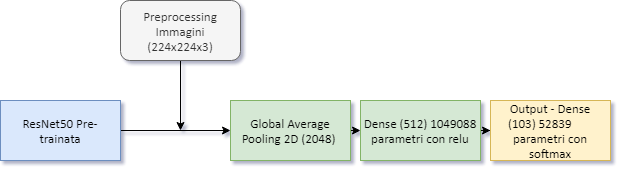
\includegraphics[width=1\textwidth]{./resources/AdvanceMachineLearningSchema-Esperimento1_V1.png}
    \caption{Disegno architetturale esperimento 1 Versione 1 ResNet50} 
    \label{fig:architettura-esperimento1_V1}
\end{figure}


\begin{figure}
    \centering
    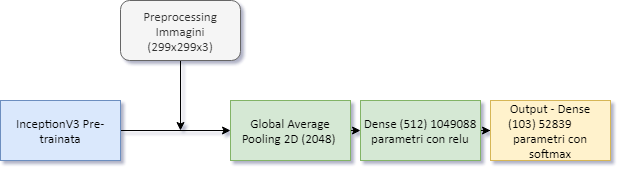
\includegraphics[width=1\textwidth]{./resources/AdvanceMachineLearningSchema-Esperimento1_V2.png}
    \caption{Disegno architetturale esperimento 1 Versione 1 InceptionV3} 
    \label{fig:architettura-esperimento1_V2}
\end{figure}

\subsection{Esperimento 2: Freeze Layers}

Nel secondo esperimento si è deciso di utilizzare un approccio di Transfer Learning simile al primo, ma questa volta effettuando un congelamento parziale della rete, rimuovendo lo strato di classificazione finale che segue lo strato convoluzionale di feature extraction e attivando anche gli ultimi 4 layers convoluzionali.
Differentemente rispetto all'esperimento 1 è stata però considerata un altro tipo di rete: VGG16 sempre ottenuta dai modelli pre-trainati di Keras. \\
La rete utilizzata quindi ha attivi gli ultimi 4 layers convoluzionali appartenenti alla rete originale (tre layers convoluzionali e un max pooling finale), viene quindi inserito sopra ad essi una propria combinazione di layers così composti: un flattern layer a seguito della parte convoluzionale, un dense layer di 1024 unità con funzione di attivazione: Relu, un layer di Dropout con tasso equivalente a 0.5 che corrisponde alla frazione di unità di input su cui effettuare il drop e infine l'ultimo strato denso formato da 103 unità equivalenti alle classi utilizzate sul nostro dataset, usando come funzione di attivazione una relu.\\
La loss function utilizzata è una categorical crossentropy come nell'esperimento 1, mentre l'ottimizzatore impiegato è sempre un Stochastic gradient descent optimizer. \bigskip

Come ulteriore prova a sostegno di questo secondo esperimento, è stato eseguito un altro tentativo utilizzando come rete di riferimento pre-trainata non più VGG16, ma InceptionV3 sempre con i pesi relativi a ImageNet, con un input differente, in modo da adattare le immagini alla nuova rete, ma con la stessa struttura precedente. \\
L'architettura relativa all'esperimento 2 versione 1 con VGG16 è rappresentata nell'immagine \ref{fig:architettura-esperimento2_V1} , mentre l'architettura per il secondo test sempre dell'esperimento 2 è rappresentata dall'immagine \ref{fig:architettura-esperimento2_V2}

\begin{figure}
    \centering
    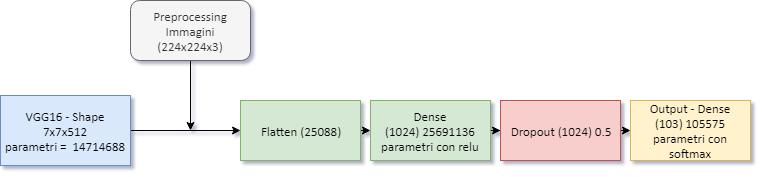
\includegraphics[width=1\textwidth]{./resources/AdvanceMachineLearningSchema-Esperimento2_V1.png}
    \caption{Disegno architetturale esperimento 2 Versione 1 con VGG16} 
    \label{fig:architettura-esperimento2_V1}
\end{figure}

\begin{figure}
    \centering
    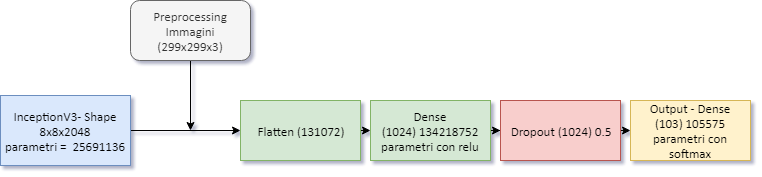
\includegraphics[width=1\textwidth]{./resources/AdvanceMachineLearningSchema-Esperimento2_V2.png}
    \caption{Disegno architetturale esperimento 2 Versione 2 con InceptionV3} 
    \label{fig:architettura-esperimento2_V2}
\end{figure}



\subsection{Esperimento 3: Implementazione rete neurale}

Dopo aver effettuato diversi esperimenti utilizzando tecniche di transfer learning si è deciso di implementare anche una rete neurale partendo dal paper di riferimento associato al dataset \cite{customnet} in modo da confrontare i risultati e verificare se un approccio completamente manuale fosse migliore rispetto all'utilizzo di reti neurali esistenti, sia in termini di facilità di realizzazione, tempo di training che di risultati effettivi. \\
Le immagini usate per il training e per la validazione sono state trattate sempre con gli stessi metodi precedenti con una risoluzione di 100x100 pixels di altezza e larghezza. \\
La configurazione della rete è illustrata nella seguente tabella: \\

\begin{table}
    \centering
    \begin{tabular}{|l|l|l|}
    \hline
    \textbf{Layer Type} & \textbf{Dimension} & \textbf{Output} \\ \hline
    Convolutional   & 5 x 5 x 4         & 16     \\ \hline
    Max Pooling     & 2 x 2 - Stride 2  & -      \\ \hline
    Convolutional   & 5 x 5 x 16        & 32     \\ \hline
    Max Pooling     & 2 x 2 - Stride 2  & -      \\ \hline
    Convolutional   & 5 x 5 x 32        & 64     \\ \hline
    Max Pooling     & 2 x 2 - Stride 2  & -      \\ \hline
    Convolutional   & 5 x 5 x 64        & 128    \\ \hline
    Max Pooling     & 2 x 2 - Stride 2  & -      \\ \hline
    Fully Connected & 5 x 5 x 128       & 1024   \\ \hline
    Fully Connected & 1024              & 256    \\ \hline
    Softmax         & 256               & 60     \\ \hline
    \end{tabular}
    \caption{\label{tab:esperimento3_configurazione}Tabella di configurazione della rete neurale convoluzionale creata a mano}
\end{table}

Per il modello utilizzato sono state impiegate come funzione di loss: categorical crosse ntropy in quanto i nostri target da predirre sono 103 classi categoriche numeriche tramite softmax. Come ottimizzatore si è scelto di utilizzare: adam ovvero adaptive moment estimation che ha risultati migliori rispetto ad altri metodi stocastici di ottimizzazione \cite{adam}.

Il disegno architetturale della rete implementata con le relative specifiche strutturali è rappresentato dall'immagine \ref{fig:architettura-esperimento3}
\begin{figure}
    \centering
    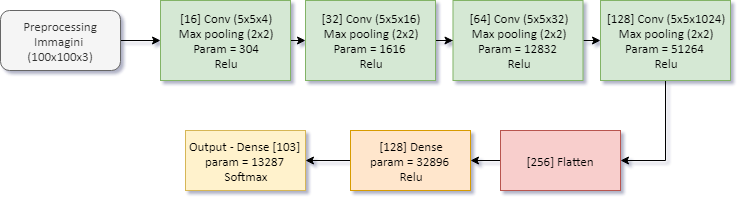
\includegraphics[width=1\textwidth]{./resources/AdvanceMachineLearningSchema-Esperimento3.png}
    \caption{Disegno architetturale esperimento 3} 
    \label{fig:architettura-esperimento3}
\end{figure}




\section{Risultati e valutazione}

Vengono quindi riportate le soluzioni e i risultati ottenuti conseguentemente all'apprendimento degli algoritmi.

\subsection{Esperimento 1}


\subsubsection{Versione 1}
Per l'esperimento 1 sono stati ottenuti i seguenti risultati 

\begin{table}[H]
    \begin{tabular}{|l|l|l|}
    \hline
    \textbf{Dataset}     & \textbf{Accuracy}           & \textbf{Loss}                 \\ \hline
    Trainingset & 0.9983263440961317 & 0.01822905129225315  \\ \hline
    Validation  & 0.9963575231157187 & 0.011467085026564319 \\ \hline
    \end{tabular}
   	 \caption{\label{tab:esperimento1_v1_risultati}Tabella dei risultati dell'esperimento 1 versione 1 con ResNet50}
\end{table}

\begin{figure}[H]
    \begin{subfigure}[b]{0.5\textwidth}
        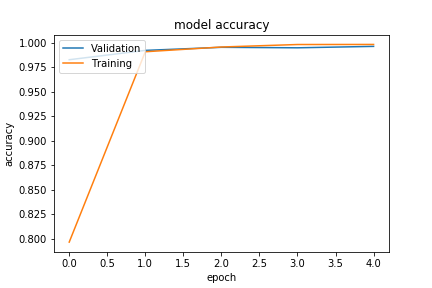
\includegraphics[width=\textwidth]{./plots/exp1_p1_bestmodel_acc.png}
        \caption{Esperimento 1 v1, risultati accuratezza} 
        \label{fig:plot_exp1_p1_acc}
    \end{subfigure}
    \begin{subfigure}[b]{0.5\textwidth}
        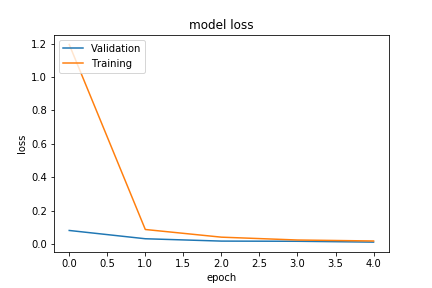
\includegraphics[width=\textwidth]{./plots/exp1_p1_bestmodel_loss.png}
        \caption{Esperimento 1 v1, risultati loss} 
        \label{fig:plot_exp1_p1_loss}
	\end{subfigure}
\end{figure}

Il tempo di training della rete sull'architettura hardware utilizzata è di:

\subsubsection{Versione 2}
Per l'esperimento 1 versione 2, usando la rete pre-trainata InceptionV3 definita precedentemente sono stati ottenuti i seguenti risultati

\begin{table}[H]
    \begin{tabular}{|l|l|l|}
    \hline
    \textbf{Dataset}     & \textbf{Accuracy}           & \textbf{Loss}                 \\ \hline
    Trainingset & 0.9967091035598097 & 0.04332224593808697  \\ \hline
    Validation  & 0.9947884561501821 & 0.019240403047854925 \\ \hline
    \end{tabular}
   	 \caption{\label{tab:esperimento1_v2_risultati}Tabella dei risultati dell'esperimento 1 versione 2 con InceptionV3}
\end{table}

Mentre i grafici relativi all'andamento delle performance rispetto al numero di epoche utilizzate sono i seguenti
\begin{figure}[H]
    \begin{subfigure}[b]{0.5\textwidth}
        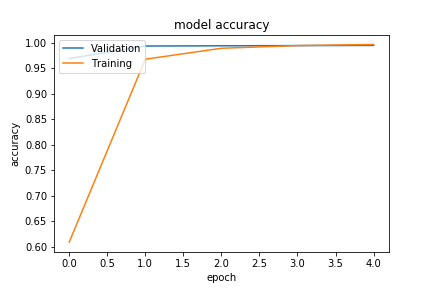
\includegraphics[width=\textwidth]{./plots/exp1_p2_acc.png}
        \caption{Esperimento 1 v2, risultati accuratezza} 
        \label{fig:plot_exp1_p2_acc}
    \end{subfigure}
    \begin{subfigure}[b]{0.5\textwidth}
        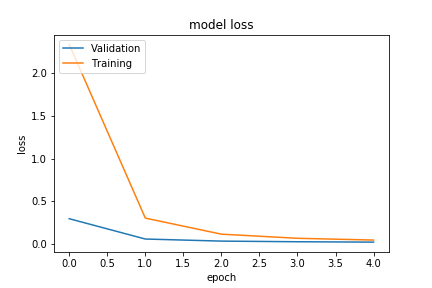
\includegraphics[width=\textwidth]{./plots/exp1_p2_loss.png}
        \caption{Esperimento 1 v2, risultati loss} 
        \label{fig:plot_exp1_p2_loss}
	\end{subfigure}
\end{figure}
Il tempo medio di training di una rete sull'architettura hardware utilizzata è di circa due ore e 30 minuti, mentre il modello in formato onnx su disco pesa: all'incirca 200 MB in entrambi i casi.

\subsection{Esperimento 2}

\subsubsection{Versione 1}
Per l'esperimento 2 versione 1, usando la rete pre-trainata VGG16 definita precedentemente sono stati ottenuti i seguenti risultati
\begin{table}[H]
    \begin{tabular}{|l|l|l|}
    \hline
    \textbf{Dataset}     & \textbf{Accuracy}           & \textbf{Loss}                 \\ \hline
    Trainingset & 0.9935310378547116 & 0.023791958318985264 \\ \hline
    Validation  & 0.9924908938077893 & 0.02455971877568624  \\ \hline
    \end{tabular}
   	\caption{\label{tab:esperimento2_v1_risultati}Tabella dei risultati dell'esperimento 2 versione 1 con VGG16}
\end{table}

Mentre i grafici relativi all'andamento delle performance rispetto al numero di epoche utilizzate sono i seguenti

\begin{figure}[H]
    \begin{subfigure}[b]{0.5\textwidth}
        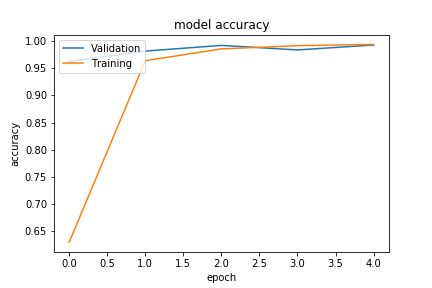
\includegraphics[width=\textwidth]{./plots/exp2_p1_acc.png}
        \caption{Esperimento 2 v1, risultati accuratezza} 
        \label{fig:plot_exp2_p1_acc}
    \end{subfigure}
    \begin{subfigure}[b]{0.5\textwidth}
        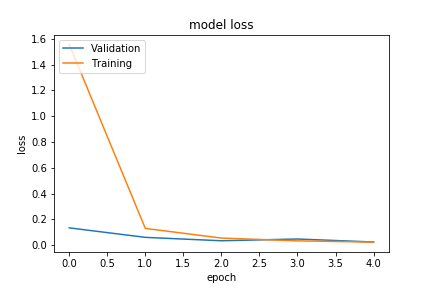
\includegraphics[width=\textwidth]{./plots/exp2_p1_loss.png}
        \caption{Esperimento 2 v1, risultati loss} 
        \label{fig:plot_exp2_p1_loss}
	\end{subfigure}
\end{figure}
Il tempo di training della rete sull'architettura hardware utilizzata è di:

\subsubsection{Versione 2}
Per l'esperimento 2 versione 2, usando la rete pre-trainata InceptionV3 definita precedentemente sono stati ottenuti i seguenti risultati
\begin{table}[H]
    \begin{tabular}{|l|l|l|}
    \hline
    \textbf{Dataset}     & \textbf{Accuracy}           & \textbf{Loss}                 \\ \hline
    Trainingset & 0.9823796002030953 & 0.06881602044664113 \\ \hline
    Validation  & 0.3503502381636202 & 2.6863035547729965  \\ \hline
    \end{tabular}
   	\caption{\label{tab:esperimento2_v2_risultati}Tabella dei risultati dell'esperimento 2 versione 2 con InceptionV3}
\end{table}

Mentre i grafici relativi all'andamento delle performance rispetto al numero di epoche utilizzate sono i seguenti
\begin{figure}[H]
    \begin{subfigure}[b]{0.5\textwidth}
        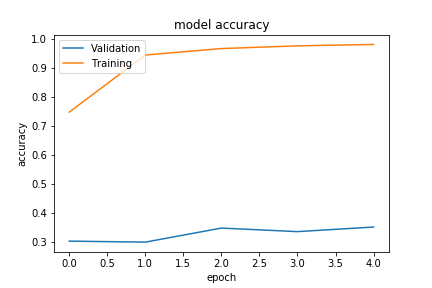
\includegraphics[width=\textwidth]{./plots/exp2_p2_acc.png}
        \caption{Esperimento 2 v2, risultati accuratezza} 
        \label{fig:plot_exp2_p2_acc}
    \end{subfigure}
    \begin{subfigure}[b]{0.5\textwidth}
        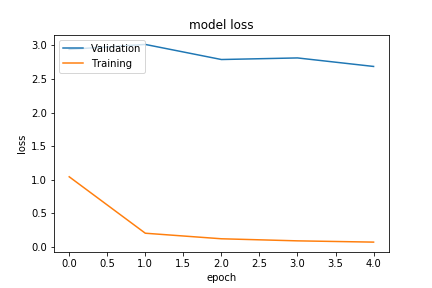
\includegraphics[width=\textwidth]{./plots/exp2_p2_loss.png}
        \caption{Esperimento 2 v2, risultati loss} 
        \label{fig:plot_exp2_p2_loss}
	\end{subfigure}
\end{figure}
Il tempo medio di training di una rete sull'architettura hardware utilizzata è di circa quattro ore, mentre il modello in formato onnx su disco pesa: all'incirca 160 MB in entrambi i casi.


\subsection{Esperimento 3}

Per l'esperimento 3 realizzato con la rete costruita artigianalmente e definita precedentemente sono stati ottenuti i seguenti risultati

\begin{table}[H]
    \begin{tabular}{|l|l|l|}
    \hline
    \textbf{Dataset}     & \textbf{Accuracy}           & \textbf{Loss}                 \\ \hline
    Trainingset & 0.964025800629212 & 0.11182551736345149 \\ \hline
    Validation  & 0.9247408237601569 & 0.323432678943311  \\ \hline
    \end{tabular}
   	\caption{\label{tab:esperimento3_risultati}Tabella dei risultati dell'esperimento 3 con la rete costruita artigianalmente}
\end{table}

\begin{figure}[H]
    \begin{subfigure}[b]{0.5\textwidth}
        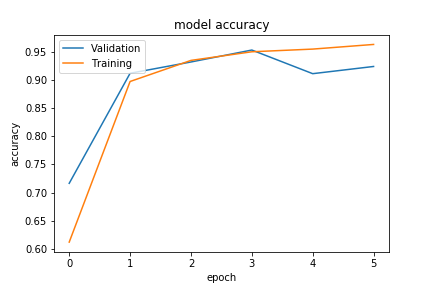
\includegraphics[width=\textwidth]{./plots/exp3_p1_acc.png}
        \caption{Esperimento 3, risultati accuratezza} 
        \label{fig:plot_exp3_p1_acc}
    \end{subfigure}
    \begin{subfigure}[b]{0.5\textwidth}
        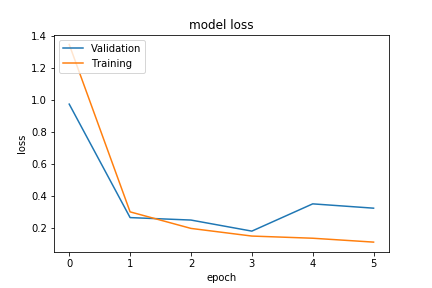
\includegraphics[width=\textwidth]{./plots/exp3_p1_loss.png}
        \caption{Esperimento 3, risultati loss} 
        \label{fig:plot_exp3_p1_loss}
	\end{subfigure}
\end{figure}

Il tempo medio di training della rete sull'architettura hardware utilizzata è di circa tre ore, mentre il modello in formato onnx su disco pesa: 443 KB

Nel secondo esperimento dire che ci sono problemi di: forgetting.
All'epoca 1 e 2 ho un salto sulla loss, in questo momento quindi il modello sta overfittando.  
Per superare questo problema è necessario fare: gradual unfreezing.  
Altra tecnica: chain-thaw.  
I primi esempi hanno un errore molto alto, iniziano a fare back propagation e cambia tanto la rappresentazione astratta.

Terzo modello, risultati buoni e interessanti, non tanto quanto transfer learning normale.


\section{Discussione dei risultati}

I risultati ottenuti dalle reti sul dataset utilizzato sono molto soddisfacenti, sia in termini di accuratezza che in termini di loss.
Si riportano le due tabelle comparative finali con i risultati ottenuti da tutte le reti impiegate negli esperimenti \ref{tab:confronto_risultati_training} \ref{tab:confronto_risultati_loss}

\begin{table}[H]
    \begin{tabular}{|l|l|l|l|l|}
    \hline
    \textbf{Rete}                         & \textbf{Training acc} & \textbf{Training loss}   \\ \hline
    Exp1, ResNet50     & 0.9967091035598097     & 0.04332224593808697 \\ \hline
    Exp1, InceptionV3  & 0.9967091035598097     & 0.04332224593808697  \\ \hline
    Exp2, VGG16        & 0.9935310378547116     & 0.023791958318985264  \\ \hline
    Exp2, InceptionV3  & 0.9823796002030953     & 0.06881602044664113   \\ \hline
    Exp3, Custom Model & 0.964025800629212      & 0.11182551736345149     \\ \hline
    \end{tabular}
    \caption{\label{tab:confronto_risultati_training}Confronto dei risultati ottenuti sul trainingset tra tutti i modelli}
\end{table}

\begin{table}[H]
    \begin{tabular}{|l|l|l|l|l|}
    \hline
    \textbf{Rete}                         &  \textbf{Validation acc} & \textbf{Validation loss}    \\ \hline
    Exp1, ResNet50      & 0.9947884561501821    & 0.019240403047854925 \\ \hline
    Exp1, InceptionV3  & 0.9947884561501821    & 0.019240403047854925 \\ \hline
    Exp2, VGG16        & 0.9924908938077893    & 0.02455971877568624  \\ \hline
    Exp2, InceptionV3 & 0.3503502381636202    & 2.6863035547729965   \\ \hline
    Exp3, Custom Model  & 0.9247408237601569    & 0.323432678943311    \\ \hline
    \end{tabular}
    \caption{\label{tab:confronto_risultati_loss}Confronto dei risultati ottenuti sul validation set tra tutti i modelli}
\end{table}

Dalle tabelle e dai valori di training e loss possiamo evidenziare come le reti ottenute grazie al primo esperimento di transfer learning, utilizzando le reti così come sono state salvate, sono sicuramente migliori rispetto agli altri approcci utilizzati, anche se con piccole differenze.
Ci sono grandi differenze invece riguardo ai tempi di training e al peso dei modelli finali una volta esportati in formato onnx.  
Il modello più leggero in termini di spazio occupato su disco è sicuramente la rete ottenuta grazie all'implementazione custom che però presenta dei valori di loss più alti rispetto agli altri modelli.
Questo parametro di confronto di spazio su disco è molto importante perchè ci permette di identificare un modello leggero e performante da poter utilizzare su numerose applicazioni, soprattutto in ambito mobile.  \bigskip

È comunque interessante contestualizzare anche i grafici di loss e accuracy presentati nel capitolo precedente per l'esperimento 2, rispetto all'esperimento 1.  
Nonostante il numero di epoche impiegate sia basso per l'esperimento 2 possiamo constatare come, nell'esperimento 2 versione 2 utilizzando InceptionV3, i risultati siano profondamente differenti in termini di performance sul validation set rispetto all'esperimento 2 versione 1 e rispetto all'esperimento 1.  
Questo comportamento è sicuramente causato dal basso numero di epoche impiegato su una rete molto più grande di VGG16 impiegata nella versione 1 dell'esperimento 2.
Avendo a disposizione una rete più grande e complessa è necessario utilizzare un tempo di training superiore, su un numero di epoche superiore oltre che ad aumentare la profondità di layer non congelati in modo da favorire l'aggiornamento di ulteriori layers rispetto alle immagini impiegate. \bigskip

È interessante notare come nell'esperimento 3 ci sia al crescere delle epoche un leggero overfitting sul validation test rispetto al training. Sicuramente un tuning degli iperparametri utilizzati dalla rete potrebbe essere di grande aiuto nell'ottimizzare le performance generali.

\subsection{Valutazione degli errori}

Considerando i modelli impiegati nell'esperimento 1 e nell'esperimento 3 è importante validare ed evidenziare quali sono gli errori all'interno del validation set utilizzato per verificare le performance del modello.
In questo modo si è in grado di definire su quali immagini i modelli sbagliano più frequentemente e per quale tipo di input.

Il numero di immagini valutate non correttamente per l'esperimento 1 su una predizione del validation set è di 47 su 17845 immagini.
Il rapporto di errori di classificazione sempre sullo stesso dataset per l'esperimento 3 è di 53 su 17845 immagini.

Alcuni esempi di immagini non correttamente classificate sono le seguenti (in entrambi i casi):

\begin{figure}[H]
    \centering
    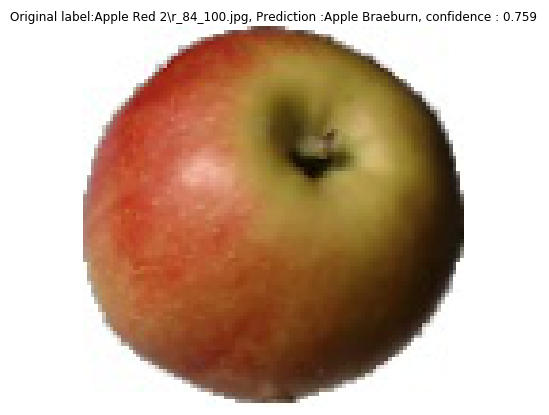
\includegraphics[width=0.3\textwidth]{./resources/error1.png}
    \caption{Errore nella predizione: ground truth: Apple Red 2, prediction: Apple Braeburn, confidenza: 0.759} 
    \label{fig:mela}
\end{figure}

\begin{figure}[H]
    \centering
    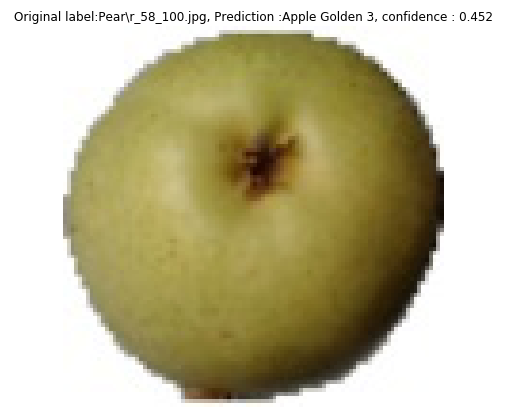
\includegraphics[width=0.3\textwidth]{./resources/error2.png}
    \caption{Errore nella predizione: ground truth: Pear, prediction: Apple Golden 3, confidenza: 0.452} 
    \label{fig:mela}
\end{figure}

\begin{figure}[H]
    \centering
    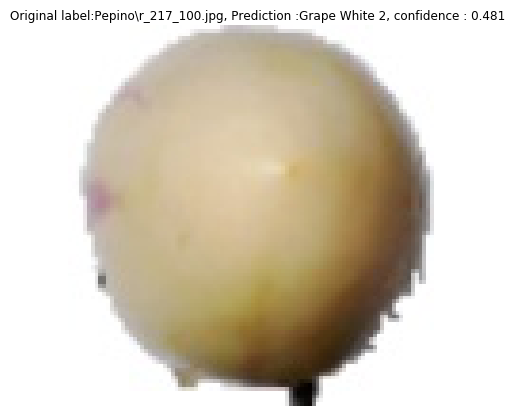
\includegraphics[width=0.3\textwidth]{./resources/error3.png}
    \caption{Errore nella predizione: ground truth: Pepino, prediction: Grape White 2, confidenza: 0.481} 
    \label{fig:error3}
\end{figure}

\begin{figure}[H]
    \centering
    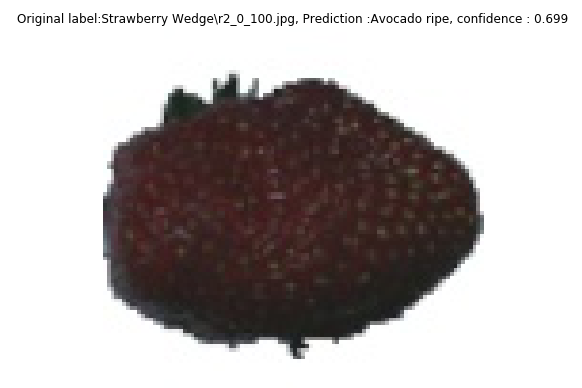
\includegraphics[width=0.3\textwidth]{./resources/error4.png}
    \caption{Errore nella predizione: ground truth: Strawberry Wedge, prediction: Avocado pipe , confidenza: 0.699} 
    \label{fig:error4}
\end{figure}

\subsection{Sviluppi futuri}

Gli esperimenti di transfer learning hanno dato degli ottimi risultati, c'è ancora ampio spazio di miglioramento per quanto riguarda i modelli trattati nell'esperimento 2. Per quanto riguarda l'esperimento 3 invece un progressivo fine-tuning dei parametri del modello potrebbe aiutare molto nel generare delle performance migliori rispetto a quanto ottenuto con i primi test e quindi generare un modello definitamente più ottimale e funzionale per qualsiasi tipo di applicazione.
Il successivo passo dopo questa sperimentazione sarà l'implementazione di un'architettura end-to-end di rilascio dei modelli in modo da favorire il loro utilizzo su diversi dispositivi, risultato ottenibile grazie all'implementazione in fase di training del salvataggio dei modelli in formato onnx.
L'implementazione di questa architettura potrebbe essere di grande vantaggio per la realizzazione di macchinari in grado di distinguere la frutta da raccogliere all'interno di frutteti e campi consentendo, attraverso l'uso di appositi macchinari, la raccolta automatizzata dei prodotti agroalimentari.
Potrebbe essere infine utile una sperimentazione con altri modelli pre trainati in modo da condurre un test più accurato e di larga scala anche su approcci differenti che potrebbero fornire risultati migliori rispetto a quelli impiegati per questo test.


\section{Conclusioni}

Gli esperimenti compiuti con le procedure di transfer learning hanno dato degli ottimi risultati. Le tecniche utilizzate sono sicuramente un utile e valido approccio per costruire ottimi modelli velocemente e con bassa capacità di calcolo, anche se il rischio di overfitting è sempre presente e bisogna prestare molta attenzione all'adattabilità con il proprio dataset, il proprio dominio e le proprie classi, in base al modello scelto. \\
L'implementazione manuale del modello basata sul paper di riferimento ha dato dei buoni risultati comparativamente ai modelli riutilizzati, il problema è che il tempo di training e le risorse richieste sono comunque più alte rispetto alle tecniche di Transfer Learning trattate con il primo esperimento.
La soluzione artigianale comunque ha rivelato buone performance e una rete più piccola e snella in grado di adattarsi bene a contesti in cui è importante avere dei modelli funzionali impiegabili su determinati casi d'uso e pratici come la realizzazione di un'applicazione web o mobile che necessita di performance sufficienti ma poco spazio occupato oppure nell'utilizzo di sistemi embedded. \\
Lo standard onnx adottato e sperimentato per salvare le reti si è rivelato un approccio vincente per l'operazionalizzazione dei processi di training e prediction, unico aspetto negativo è la poca adattabilità con il framework di Keras per quanto riguarda la fase di prediction.
Nel complesso, le soluzioni adottate e le architetture impiegate si sono rivelate corrette per rispondere alla domanda iniziale, ovvero trovare delle tecniche in grado di classificare correttamente differenti tipi di frutta a partire da immagini.


\bibliographystyle{IEEEtran}
\bibliography{references.bib}

\end{document}